\documentclass{report}
\usepackage{preamble}

\begin{document}
\bibliographystyle{plainurl}% the mandatory bibstyle

\begin{titlepage}
  \centering
  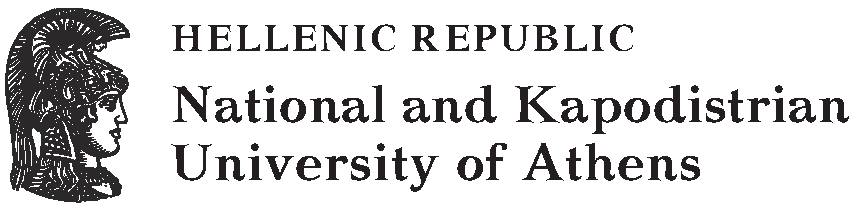
\includegraphics[width=\textwidth]{figures/uoa.pdf}\par\vspace{1cm}
  {\scshape\Large Department of Computer Science\par}
  \vspace{1cm}
  {\scshape A dissertation submitted for the degree of Doctor of Philosophy\par}
  \vspace{1cm}
  {\huge\bfseries Decentralized Cross-Chain Communication Mechanisms for Proof-of-Work and Proof-of-Stake Blockchains\par}
  \vspace{2cm}
  {\Large\itshape Dionysis Zindros\par}
	\vfill
	{\large \today\par}
\end{titlepage}

\newpage

\thispagestyle{empty}
\null

\newpage

\begin{abstract}
During the last decade, the blockchain space has exploded with a plethora of new cryptocurrencies, covering a wide array of different features, performance and security characteristics. Nevertheless, each of these coins functions in a stand-alone manner, independently.  Sidechains have been envisioned as a mechanism to allow blockchains to communicate with one another and, among other applications, allow the transfer of value from one chain to another, but so far there have been no decentralized constructions.

In this thesis, we explore the question of whether it is possible to build interoperability between blockchains and allow them to communicate. Interoperability stands as a stepping stone to enable the solution of problems that have remained important open questions in the blockchain space for years, including interfacing with legacy monetary systems, upgradability, scalability and sustainability. We put forth the first sidechains construction that allows communication between proof-of-stake and proof-of-work blockchains, and combinations thereof, without trusted intermediaries.

In the heart of our sidechains constructions stand two new cryptographic primitives which we introduce in this work. On the proof-of-stake side, the ATMS primitive (Ad-Hoc Threshold Multisignatures) allows attesting to the shifting of stake from epoch to epoch. We provide the first ATMS construction. On the proof-of-work side, the NIPoPoWs primitive (Non-Interactive Proofs of Proof-of-Work) allows compressing proof-of-work into succinct strings that shrink a long blockchain into a single proof. We provide the first NIPoPoWs construction.

We give formal proofs of security for our constructions. In the proof-of-work side, we first explore the setting of constant difficulty and prove our construction secure there. We subsequently analyze our protocol and prove it secure in the variable difficulty setting. In the proof-of-stake side, we require bounded stake-shifting. We assume honest work majority for proof-of-work and honest stake majority for proof-of-stake. Our analysis is in the synchronous setting. Our analysis is cryptographic and our security is proven with overwhelming probability against all polynomial adversaries. For NIPoPoWs, our proof is by reduction to the security of the underlying blockchain and is based on the Bitcoin Backbone model in the Random Oracle model. Our proof-of-work sidechain construction is proven secure by reduction to the security of NIPoPoWs. Our proof-of-stake sidechain construction is studied in the Ouroboros setting and is proven secure by reduction to the security of ATMS.

Our constructions are generic in that we allow the passing of any information between blockchains. Our cross-chain certificates allow proving general predicates about blockchains which can encode any generic events within a blockchain. Thus, our sidechain construction is not limited to the exchange of assets and value.

Our NIPoPoWs and ATMS primitives have more applications beyond sidechains, including the introduction of blockchain clients that have small communication complexity and are non-interactive and are thus superlight. For the proof-of-work case, our proofs are polylogarithmic in the size of the chain. For the proof-of-stake case, our proofs are linear in the number of epochs. We are the first to put forth such superlight client protocols which improve upon the known SPV protocols. Our sidechain constructions have various applications, two prominent examples of which are the ``remote ICO,'' in which an investor pays in currency on one blockchain to receive tokens in another, and the ``two-way peg,'' in which an asset can be transferred from one chain to another and back.

We provide numerous experiments, simulations and implementations illustrating the feasibility of our scheme, including measurements of security and performance metrics and give concrete proposals for the security parameters to be used by our schemes in practice. We demonstrate the feasibility of our construction by providing an implementation in the form of a Solidity smart contract. Our cross-chain protocols have already been implemented in real-world deployments of blockchains by third parties, including ERGO, nimiq, WebDollar for proof-of-work and Cardano for proof-of-stake.

% Future work: we will consider the security of our construction in a semi-synchronous setting. We will also explore the feasibility of various sidechain topologies and the challenges occurring throughout the lifecycle of a blockchain and its sidechains, from the birth of a sidechain where honest majority is difficult to achieve, to the death of a blockchain in which its assets need to be migrated to new blockchains. Last, we will provide full production implementations for both proof-of-stake (in the Cardano cryptocurrency) and in proof-of-work (in the Ethereum, Ethereum Classic and Bitcoin Cash) settings, as well as hybrid settings.
\end{abstract}

\newpage

\tableofcontents

\newpage

% TODO: list of figures, list of tables
\chapter*{Preface}
\addcontentsline{toc}{chapter}{Preface}

% structure of the thesis
% acknowledgements

\chapter{Introduction}\label{chapter:introduction}

\todo{Fill in introduction...}

Bitcoin \index{Bitcoin}\cite{bitcoin}

\section{Motivation}
% superlight clients
% sidechains
\section{Our Contributions}
\section{Related Work}
% KLS
% other sidechains works
% - omniledger
% - rootstock
% - Todd sidechains
% - xclaim
% - rootstock
% - polkadot
% - truebit?
% - flyclient

\chapter{Background}

% bitcoin

\chapter{Proofs of Proof-of-Work}\label{chapter:work}

\cite{nipopows}

\section{Blockchain Proofs}
\subsection{The Prover/Verifier Model}
\subsection{Provable Chain Predicates}
\subsection{Desired Properties}

\section{Superblocks}
\section{Suffix Proofs}
\section{Infix Proofs}
\section{Superchain Quality} % or growth?
\section{An Attack}
\section{Security}
\section{Succinctness}
\section{Implementation Parameters}
\section{Velvet Forks and Deployment Paths}

\chapter{Proofs of Proof-of-Stake}\label{chapter:stake}

\section{Ad-Hoc Threshold Multisignatures}
\section{ATMS Constructions}

\chapter{Sidechains}

\section{Validity Languages}
\section{Deployment Options}
% direct observation, agnosticism etc. here
\section{Sidechain Lifecycle}
\section{Sidechain Security}
\section{Certificate Transactions}
\section{Direct Construction}
\section{Security}
\section{Smart Contract Construction}

% lite clients?
\chapter{Conclusion}\label{chapter:conclusion}

Throughout this thesis, we have presented effective consensus compression
mechanisms for all decentralized blockchain protocols, in particular for
both proof-of-work and proof-of-stake. We introduced the NIPoPoWs primitive for
proof-of-work and the ATMS primitive for proof-of-stake. For proof-of-work, we
presented the following variants:

\begin{itemize}
  \item \emph{Charity with goodness} in the static synchronous model, which
        achieves security against a $\frac{1}{2}$ adversary, but succinctness
        only optimistically.
  \item \emph{Charity without goodness} which achieves both security and
        succinctness against a $\frac{1}{3}$ adversary in both the static and
        variable synchronous models and achieves both security and succinctness
        against a $\frac{1}{4}$ adversary in both the static and variable
        $\Delta$-bounded delay model. Succinctness is achieved when difficulty
        does not decrease exponentially.
  \item \emph{Distill}, which achieves comparable results to the above, with the
        additional assumption that difficulty is non-decreasing.
\end{itemize}

For the first among the above, we gave concrete security parameters obtained
through experimental analysis and simulations.

We gave three important applications of our primitives:

\begin{itemize}
  \item \emph{Superlight clients}, which allow the construction of wallets that
        can synchronize faster than standard SPV wallets. The improvement is
        exponential for proof-of-work and constant for proof-of-stake.
  \item \emph{Logarithmic space mining}, which allows the replacement of all
        proof-of-work miners of the protocol with logarithmic-space equivalents
        under the assumption that honest $\frac{1}{4}$ majority holds always.
        The improvement is exponential compared to standard miners for both
        state as well as communication complexity.
  \item \emph{Blockchain interoperability}, which allows any variant of
        blockchains to communicate, namely work/work, work/stake and
        stake/stake. We gave constructions using native support (for stake) as
        well as smart contract-based constructions (for work) and showed how
        they can be used for generic information transfer. Finally, we leveraged
        them to construct one-way and two-way pegs.
\end{itemize}

In addition to improving efficiency of existing solutions, our constructions
hint towards two avenues which are in need of improvement in the blockchain
space more generally. The first avenue concerns \emph{scalability}, a major
current topic of research in the field. While most solutions have been focusing
on layer-2 solutions such as Lightning~\cite{lightning}, our solution of
allowing multiple chains to interoperate and in particular our proposal to
separate the notion of a \emph{cryptocurrency} from its native \emph{blockchain}
allows sidechains to be used to offload transaction traffic off of a main chain
and into multiple sidechains. As long as the majority of transactions remain
within one chain and are not cross-chain transactions, sidechain solutions can
improve the scalability of the main chain. One example means of ensuring sharded
transaction traffic is to create one sidechain per particular industry or
wide geographical location. The second avenue concerns \emph{upgradability} and
the trial of new features. While soft forks and hard forks require consensus
change and may face opposition, sidechains can be used to trial out new features
without requiring all of the main chain to upgrade to these new features. This
can be useful for beta-testing, but also for adopting features that are
considered more risky by the majority. The portion of the population willing to
take the risk can move their capital to a novel sidechain, while the risk-averse
majority can leverage the firewall property to protect their capital on the main
chain.

Overall, our proposals have given rise to vibrant new research directions and
have inspired solutions which are seeing practical adoption across the
cryptocurrency space. Multiple production cryptocurrencies have adopted our
protocols, among others ERGO, nimiq, and WebDollar. Lastly, our primitives have
been implemented and extended by researchers in peer reviewed papers. One
prominent example is FlyClient~\cite{flyclient}, which provides an alternative
implementation to our NIPoPoW primitive.

\section{Future Work}

As we have seen, the consensus compression primitives have numerous important
applications which can have significant impact in the space. For these to be
deployable in practice with confidence, more research is needed around the
primitives. Around the topic of proof-of-stake sidechains, the central question
that remains is whether it is possible to do so succinctly, i.e., in
$\bigO(polylog(|\chain|))$. For NIPoPoWs, more research is needed to establish
how much the model in which they achieve security can be relaxed.

We identify three major directions for future work, which we summarize below.

\textbf{Velvet NIPoPoWs.} In Chapter~\ref{chapter:work}, we discussed various
deployment strategies for NIPoPoWs and we pointed out that deployment can be
made using a hard fork, a soft fork, or a \emph{velvet fork}, and we described
some algorithmic modifications to our protocols which make velvet forking
possible. However, no proof of security was provided. In fact, velvet fork
security is more complicated than what it seems on the surface. At first
glance it seems that the adversary cannot benefit from including incorrect
pointers: She can only include either altogether \emph{wrong} pointers, or
pointers that point to the correct superblock level but are not the most recent
superblock. The first ones can be filtered out by the verified who can check the
hash of the superblock pointer. As for the wrong ones, it seems that the
adversary can only submit pointers to older blocks in the same chain, which
would only harm their success rate. However, upon closer inspection one observes
the following interesting attack: The adversary is able to include pointers not
only to older superblocks of the correct level \emph{on the same chain}, but
also on different chains. These blocks, although they have necessary been
created prior to the block in which their pointer is included, may not be
ancestors of the block in question. This allows the adversary to play a game of
\emph{chain sewing} by ``cutting'' and ``pasting'' chunks of the honestly
generated chain into their dishonest fork. This cutting and pasting allows the
velvet adversary to ``borrow'' proof-of-work from an honest chain which does not
belong to its adversarial fork, making it potentially win when compared against
an honest fork. In short, the tree containing all interlink pointers does not
look like a tree at all in the velvet case, but it forms a Directed Acyclic
Graph. Patching the protocol and proving security under these settings is
challenging and is explored in follow-up work~\cite{velvet-nipopows}.

\textbf{NIPoPoWs under dishonest majority.} While our analysis has used the
assumption that honest majority holds for \emph{all} rounds, it is a known
result that full nodes in proof-of-work settings can withstand
temporary dishonest majority~\cite{dishonest}. More specifically, consider an
execution in which honest majority holds \emph{most} of the time, but a spike of
dishonest majority occurs for a limited number of rounds. The short period of
dishonest majority is then followed by a much longer period of honest majority.
While the ledger property of persistence can be lost for the duration of the
dishonest majority spike and for an additional period thereafter, the protocol
is \emph{self-healing} in that, given sufficient time during which honest
majority holds, the protocol can recover and persistence will be restored. This
stems from the fact that the \emph{common prefix} property of chains is
self-healing. A natural question that arises is whether NIPoPoWs are also
self-healing. More specifically, in a temporary dishonest execution, a NIPoPoW
verifier can be convinced to choose a chain that does not correspond to the
chain that a full node honest party would choose. For example, that chain could
be a short chain (such that the full node would reject it) with many superblocks
(such that the NIPoPoW verifier would accept it). However, it seems that such
proofs will become superseded by honestly generated proofs that correspond to
a chain adopted by an honest full node if sufficient time time with honest
majority is allowed to pass. A full proof of this security claim in the
temporary dishonest model would significantly increase our confidence in
superblock-based NIPoPoWs.

\textbf{Bribing-resilient NIPoPoWs.} One criticism of using superblocks to
construct NIPoPoWs has been the susceptibility of these proofs to
\emph{bribing}~\cite{flyclient}. The argument goes like this: While under the
honest majority assumption the distribution of superblocks within chains will be
as expected, the \emph{real} protocol does not have honest majority. Instead,
parties behave \emph{rationally} and would be happy to deviate from the honest
protocol if appropriate incentives are provided. The idea then is for the
adversary to \emph{bribe} miners in exchange for keeping high-level superblocks
withheld. Because high-level blocks are rare, the money needed to bribe these
miners will be small. More specifically, suppressing $\mu$-level superblocks
in expectation has a cost equal to the block reward multiplied by
$|C|2^{-\mu}$ which is the number of blocks that the adversary wishes
suppressed. In fact, the cost can be even less if not \emph{all} $\mu$
superblocks are suppressed. In the case of our \emph{charity with goodness}
construction, such bribes can only harm the succinctness of the proofs, not
their security. However, a harm in succinctness can translate to a harm in
security depending on the application. For example, a cross-chain smart contract
as disucussed in Chapter~\ref{chapter:sidechains} has very limited gas
available, and proofs that are $\omega(polylog(|\chain|))$ would easily exhaust
those limits. A failure of the smart contract to receive proofs would not only
cause a denial of service, but can easily have financial cost incured by the
victims. That cost can be sufficient to provide capital to an adversary for
bribing miners. On the other hand, our \emph{charity without goodness} and our
\emph{distill} constructions directly rely on good distribution of superblocks
within the chains even for security, not just for succinctness. As such, a bribe
can directly harm security, and it is not hard to imagine a rational adversary
who makes sufficient money from their attack to be able to use some of it for
bribing purposes. To fix this issue, miner rewards have to be rebalanced
according to superblock levels. As such, a $\mu$-level superblock must receive
a reward equal to $2^\mu$ times the reward of a $0$-level block. This makes
bribing for the purposes of block suppression as costly as bribing for
suppressing the whole chain. Therefore, if the participants believe the chain
itself to be secure and not bribable, the superblocks will also survive for the
same reasons. In fact, it may be possible to allocate such rewards with a soft
fork using a smart contract beneficiary. The exact mechanics needed for reward
allocation to make NIPoPoWs bribing-resilient will be explored in future work.

\section{Epilogue}

Computer science is a data-driven science in which optimization according to
some measurable metric or another always remains the main goal. In our case, we have
optimized the space and communication complexity of blockchain consensus
protocols, and this has given rise to important applications on top. In focusing
on a narrow optimization problem, it is often easy to forget that our work has
moral impact, and one has to keep in mind the moral character of cryptographic
work~\cite{moral}. In addition to the moral dilemmas of secrecy and transparency
faced by our predecessor cryptographers who worked on secure messaging and
digital signatures, as blockchain scientists we are facing broader ethical
questions which stem from the fact that the protocols we design have the
potential for enormous economic and political impact if they are ever to become
mainstream. When I began this thesis four years ago, I was, perhaps na\"ively,
extremely excited about the democratization that blockchain protocols can bring
to the world, from their promise to \emph{bank the unbanked} to the elimination
of the extravagant fees charged by private financial institutions.

Throughout the duration of this work, after studying and understanding the
topics in depth and develping new protocols, some of that initial excitement
faded and turned to partial disillusionment. This came especially through
numerous discussions and research conducted together with my colleague Dimitris
Karakostas and our findings on lack of blockchain
egalitarianism~\cite{egalitarianism} (which does not form part of the present
work). As a new scientist, naturally it is often easy to dismiss legacy systems
such as the existing monetary and banking system by focusing on their
shortcomings instead of their advantages which one often overlooks. Despite more
sober, I am still excited about the future that blockchains and decentralized
protocols can bring if we make good use of them. We shall keep working on them
with ethics in mind. Some big picture questions will keep coming up: Are our new
protocols better than the legacy system, and in which ways? Do they lack in
others? Most importantly, are we building a system which will be a net benefit
to humankind and the less fortunate in our society? Do they preserve or improve
upon egalitarianism and democracy, and in which ways exactly? These are not
exact science questions. While everyone's answers might be different, it is
imperative that we consider the questions and each of us makes their own
judgement. For in solving our mathematical equations and proving our theorems,
we must not forget the real people that our work will impact.

\appendix
\begin{appendices}

\chapter{Mathematical Background}
\section{Identities and Inequalities}

\end{appendices}


\bibliography{bibliography}
\printindex

\end{document}
